\subsubsection{Drehturm}
\begin{figure}[h!]
	\centering
	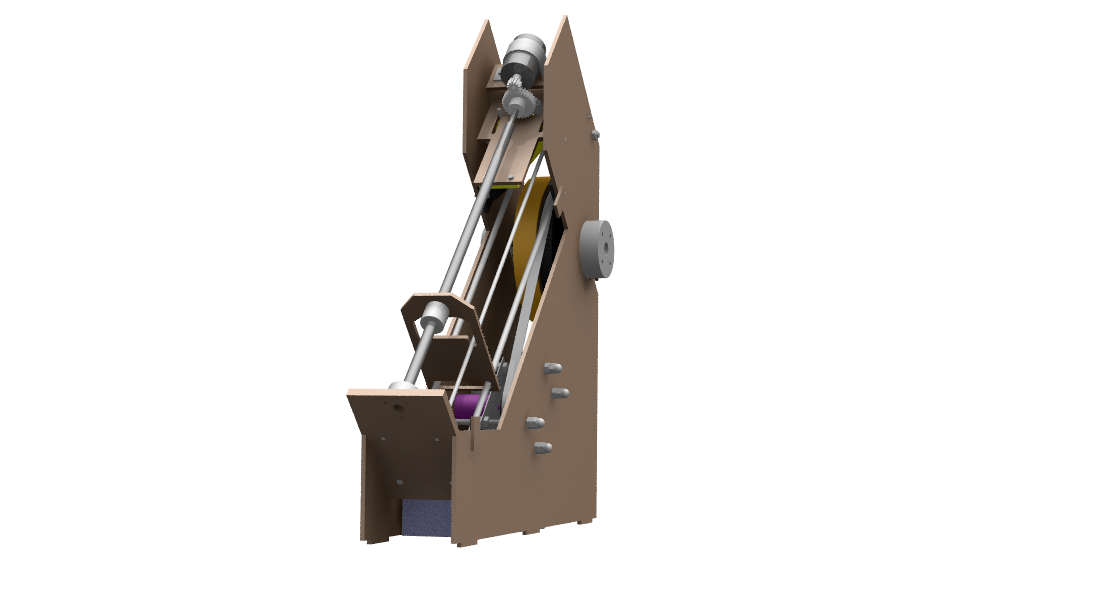
\includegraphics[width=\linewidth]{../../fig/Drehturm}
	\caption{Drehturm}
	\label{fig:Drehturm}
\end{figure}

\paragraph{Komponentenbeschrieb\\}
Der Drehturm ist das Gerüst, welches die verschiedenen Komponenten in den gewünschten Positionen hält. Er besteht aus zwei durch einen Laser zugeschnittenen MDF-Platten (Mitteldichte Holzfaserplatte) und ist durch Steckverbindungen auf dem Drehteller befestigt. Die Platten stehen parallel in einem Abstand von acht Zentimetern zueinander und umgeben somit die meisten Komponenten der Wurfmaschine. Die Vorrichtung wirkt durch diese Bauart auch ohne komplizierte Massnahmen aufgeräumt.

\paragraph{Entwicklungsprozess\\}
Schon während der frühen Entwicklungsphase des Konzeptes einigte man sich darauf, hauptsächlich durch Laserschneiden herstellbare Einzelkomponenten zu verwenden. Die Auswahl des Grundmaterials wurde daher eingeschränkt, da beispielsweise Metalle auf den Laseranlagen der Schule nur schlecht, bis gar nicht zu fertigen sind. Die Entscheidung fiel auf MDF, da dieser Werkstoff auch nach dem Laserschneiden noch gut zu bearbeiten ist. Die Form des Turmes ergab sich mehr oder weniger durch die Auswahl der Komponenten. Da ein linearer Ballnachschub gewählt wurde und die Platzverhältnisse begrenzt sind, musste in die Höhe konstruiert werden.